\documentclass{article}
\usepackage[czech]{babel}
\usepackage[utf8]{inputenc}
\usepackage{graphicx}
\usepackage{pdfpages}
\usepackage{textgreek}
\usepackage{xargs} 
\usepackage{xcolor}
\usepackage{pdfpages}
\usepackage{cite}
\usepackage[colorinlistoftodos,prependcaption,textsize=tiny]{todonotes}
\newcommandx{\xtodo}[2][1=]{\todo[linecolor=red,backgroundcolor=red!25,bordercolor=red,#1]{#2}}


\usepackage{listings}
\usepackage{color}

\definecolor{dkgreen}{rgb}{0,0.6,0}
\definecolor{gray}{rgb}{0.5,0.5,0.5}
\definecolor{mauve}{rgb}{0.58,0,0.82}

\lstset{frame=tb,
  language=Sql,
  aboveskip=3mm,
  belowskip=3mm,
  showstringspaces=false,
  columns=flexible,
  basicstyle={\small\ttfamily},
  numbers=none,
  numberstyle=\tiny\color{gray},
  keywordstyle=\color{blue},
  commentstyle=\color{dkgreen},
  stringstyle=\color{mauve},
  breaklines=true,
  breakatwhitespace=true,
  tabsize=3
}




\begin{document}


%---------------------------------------------------------------------------------------------------------------------------------------------------------------%


\begin{titlepage}	
	\begin{center}
		
\includegraphics[width=5cm]{logo.jpg}\\[3.5cm]
		{\Huge KIV/VSS}\\[0.5cm]
		{\Large 2.0. – Markovské náhodné procesy a systémy hromadné obsluhy}\\[0.5cm]
		{\large  Buffer s neomezenou kapacitou}\\[4.5cm]
		{\large  Miroslav Liška – A17N0081P}\\[0.5cm]
		{\large  topiker@students.zcu.cz}\\[0.5cm]
		{\large   9.12.1992}\\[0.5cm]
		\vfill

		{\large \today}

	\end{center}
\end{titlepage}



\section{Zadání} %%%%%%%%%%%%%%%%%%%%%%%%%%%%%%%%%%%%%%%%%%%%%%%%%%%%%%%%%%%%%%%%%%%%%%%%%%%%%%%%%%%%%%%%%%%%%%%%%%%%%%%%%%%%%%%%%%%%%%%%%%%%%%%%%%%%%%%%%%
\setcounter{page}{1}
Do bufferu s neomezenou kapacitou přicházejí zprávy, doba mezi příchodem zpráv je náhodná a má exponenciální rozdělení s parametrem \( \lambda = 9 \).
Zprávy jsou z bufferu vybírány (pokud tam nějaké jsou) opět náhodně, doba mezi po sobě jdoucími výběry zpráv je též náhodná a má exponenciální rozdělení s parametrem \( \\mu = 10 \).
S využitím markovského modelu určete:
\begin{itemize}  
\item střední počet zpráv, které se v bufferu nachází,
\item kolik procent času při dlouhodobém sledování bude buffer prázdný,
\item jak často (průměrná perioda) se buffer úplně vyprázdní. \ldots 
\end{itemize}

Pro numerický výpočet pomocí nástroje MARKOV počet stavů modelu nějak (rozumně) omezte.
 
\section{Řešení}%%%%%%%%%%%%%%%%%%%%%%%%%%%%%%%%%%%%%%%%%%%%%%%%%%%%%%%%%%%%%%%%%%%%%%%%%%%%%%%%%%%%%%%%%%%%%%%%%%%%%%%%%%%%%%%%%%%%%%%%%%%%%%%%%%%%%%%%%%


 \subsection{Model}%%%%%%%%%%%%%%%%%%%%%%%%%%%%%%%%%%%%%%%%%%%%%%%%%%%%%%%%%%%%%%%%%%%%%%%%%%%%%%%%%%%%%%%%%%%%%%%%%%%%%%%%%%%%%%%%%%%%%%%%%%%%%%%%%%%%%%%%%%

Modelem této úlohy markovský model, který má právě jednu frontu a právě jeden kanál obsluhy. 
Zpráva může do bufferu kdykoliv přijít s intenzitou \( \lambda \) a nebo být z bufferu odebrána s intenzitou \( \mu \).
Na obrázku (\ref{fig:gull})  lze vidět přechodový graf, kde čísla uvnitř zpráv reprezentují počet stavů uvnitř bufferu.

\begin{figure}[ht]
  \centering
    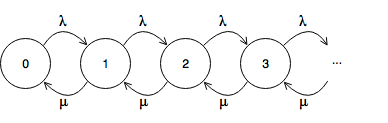
\includegraphics[width=0.6\textwidth]{vss_buffer.png}
  \caption{Přechodový model nekonečného bufferu}
  \label{fig:gull}
\end{figure}

 \subsection{Ověření zatížení systému}
Nejprve je nutné ověřit, zda je systém ve stacionárním režimu, tedy není zatížený. To lze poznat podle následujícího vzorce:
$$
	\rho = \frac{1}{m}\cdot\frac{\lambda}{\mu}
$$

Pokud vyjde \(\rho \geq 1\), znamená to, že je systém přetížený, tedy není ve stacionárním režimu a fronta neustále narůstá.

Pro zadání \( \lambda = 9 \) a \( \mu = 10 \) je \(\rho\) rovno 0,9.

\section{Implementace}
Pro implementaci je využit program MARKOV2.
\subsection{Konstrukce modelu}
Model je dán nekonečným grafem přechodů.
Pravděpodobnost stavu n lze analyticky vyjádřit jako:
$$
	p_n = (1-\rho)\rho^n
$$
Vzhledem k tomu, že je graf nekonečný, je nutné počet stavů omezit (aktuálně na 200), aby pravděpodobnost stavu byla již téměř zanedbatelná.

Skript pro jeho vytvoření vypadá následovně:\\
\newline
\texttt
{
module example [200];\\
\#define size 200\\
\#define lamda 9\\
\#define mi 10\\
\newline
for(i ;0; size-2)\{\\
	{[}i{]}->{[i+1]};\\
\}\\
\newline
for(i ;0; size-2)\{\\
	{[}i+1{]}->mi {[i]};\\
\}\\
}
\newpage
\subsection{Limitní pravděpodobnost stavů modelu}

Limitní pravděpodobnosti stavů modelu lze analyticky vyřešit řešením soustavy lineárních rovnic.

$$
0 = -\lambda p_0 + \mu p_1
$$
$$
0 =  \lambda p_0 - \mu p_1 - \lambda p_1 + \mu p_2
$$
$$
0 =  \lambda p_1 - \mu p_2 - \lambda p_2 + \mu p_3
$$
$$
\cdots
$$
$$
0 =  \lambda p_{n-1} - \mu p_{n} - \lambda p_{n} + \mu p_{n+1}
$$
$$
\cdots
$$

Pro výpis limitní pravděpodobnost s programem MARKOV2 je možné využit MMQL dotaz nad připraveným modelem. Pro přehlednost je zobrazeno prvních 10 stavů.
\newline
\newline
\texttt
{
load "example" as buf\\
define rho := 0.9;\\
select p{[i}] as ModelProb\\ 
from buf \\
for i := 0 to 9\\ 
order ModelProb desc\\
}
\newline
Výsledkem tohoto dotazu je:
\newline
\newline
\texttt
{
 ModelProb \\
 0.038742 \\
 0.0430467 \\
 0.0478297 \\
 0.0531441 \\
 0.059049 \\
 0.06561 \\
 0.0729 \\
 0.081 \\
0.09 \\
0.1 \\
}
\subsection{Výpočet středního počtu zpráv v bufferu}
Vzhledem k tomu, že model má právě jednu frontu, právě jeden kanál obsluhy a zprávy odebráné z bufferu "zmízí", je střední počet zpráv v bufferu roven střednímu počtu zpráv v systémů.
To je možné spočítat analyticky pomocí vzorce:
$$
	L_w = L_q = \frac{\rho}{1 - \rho} = \frac{0,9}{1 - 0,9}=9
$$
\newpage
\subsection{Kolik procent času při dlouhodobém sledování bude buffer prázdný}
Buffer je prázdný, pokud se nacházíme ve stavu 0. Stačí tedy získat ustálenou pravděpodobnost toho, že jsme ve stavu 0.\newline
\newline
\texttt
{
load "example" as buf\newline
select p{[0]}*100 \newline
as Prazdno from buf\newline
}
\newline
Výsledkem pak je:
\texttt
\newline
\texttt{
Prazdno \newline
10
}
\subsection{Průměrná perioda vyprázdnění bufferu}
Buffer se vyprázdní, pokud přejdeme ze stavu 1 do stavu 0. Pro výpočet periody nejprve určíme frekvenci:
$$
f_{prazdna} = p_1\mu
$$
a z frekvence následně periodu
$$
T_{prazdna} = \frac{1}{f_{prazdna}}
$$
\newline
Kód v programu MARKOV2 vypadá následovně:
\newline
\newline
\texttt
{
load "bufferexample" as buf\\
define mi := 1.0;\\
select 1/(mi*p{[1]})\\
as periodaPrazdna \\
from buf\\
}
\newline
Výsledek:
\newline
\newline
\texttt
{
periodaPrazdna\newline
11.1111
}






\section{Závěr} %%%%%%%%%%%%%%%%%%%%%%%%%%%%%%%%%%%%%%%%%%%%%%%%%%%%%%%%%%%%%%%%%%%%%%%%%%%%%%%%%%%%%%%%%%%%%%%%%%%%%%%%%%%%%%%%%%%%%%%%%%%%%%%%%%%%%%%%%%
Zadání bylo splněno ve všech bodech.
\end{document}